\section{Literature Review}
\begin{itemize}
    \item explain what a neural network is in general
    \item brief summary on how the learning works (backpropagation)
\end{itemize}

\subsection{Deep Learning Basics}
\emph{Deep Learning} is a new field of machine learning that makes use of \emph{Deep Neural Networks} (DNN)~\cite[pp.~125f]{nn_intro96}. In an abstract point of view, a DNN is just a mathematical function to map a given input vector to an output vector. It is assembled from densely-connected units called \emph{neurons} (or \emph{perceptrons}). Usually, the neurons are grouped into layers~\cite[p.~125]{nn_intro96} (see figure~\ref{fig:layered_architecture}). The first layer of the DNN has direct access to the input vector, thus it is called the \emph{input layer}. In contrast, the last layer of the DNN produces the output vector and is therefore called \emph{output layer}. In between, there is an arbitrary number of \emph{hidden layers} that make up for the depth of the neural network.

\begin{figure}[h]
    \centering
    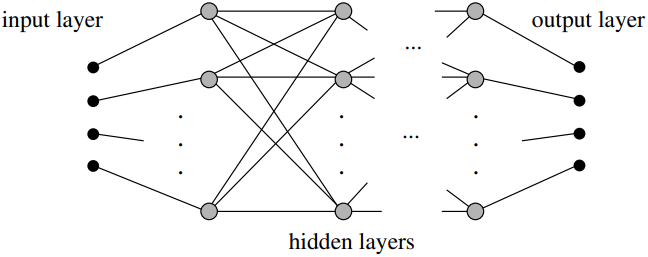
\includegraphics[width=0.7\textwidth]{images/generic_layered_architecture}
    \caption{A generic layered architecture~\cite[p.~126]{nn_intro96}}
    \label{fig:layered_architecture}
\end{figure}

Each neuron is itself a small computational unit that applies several mathematical operations, namely an \emph{input function} and an \emph{activation function}. Traditionally, the neurons of subsequent layers are densely connected, meaning a neuron of layer $k$ receives the output values from all neurons in layer $k-1$. Based on those values, the input function calculates the \emph{net input} for the neuron. In most cases this is done by using weights on the connections to perform a weighted sum over all values. The net input is then passed through the activation function whose main purpose is to break the linearity of the DNN. For the activation function there are plenty of options to choose from. An overview of commonly used function can be found in~\cite{act_funcs18} and includes for example a binary step function, a sigmoid function or rectified linear units (ReLU). Figure~\ref{fig:perceptron} depicts all the calculations done inside of a neuron.

% TODO: find/create better matching illustration
\begin{figure}[h]
    \centering
    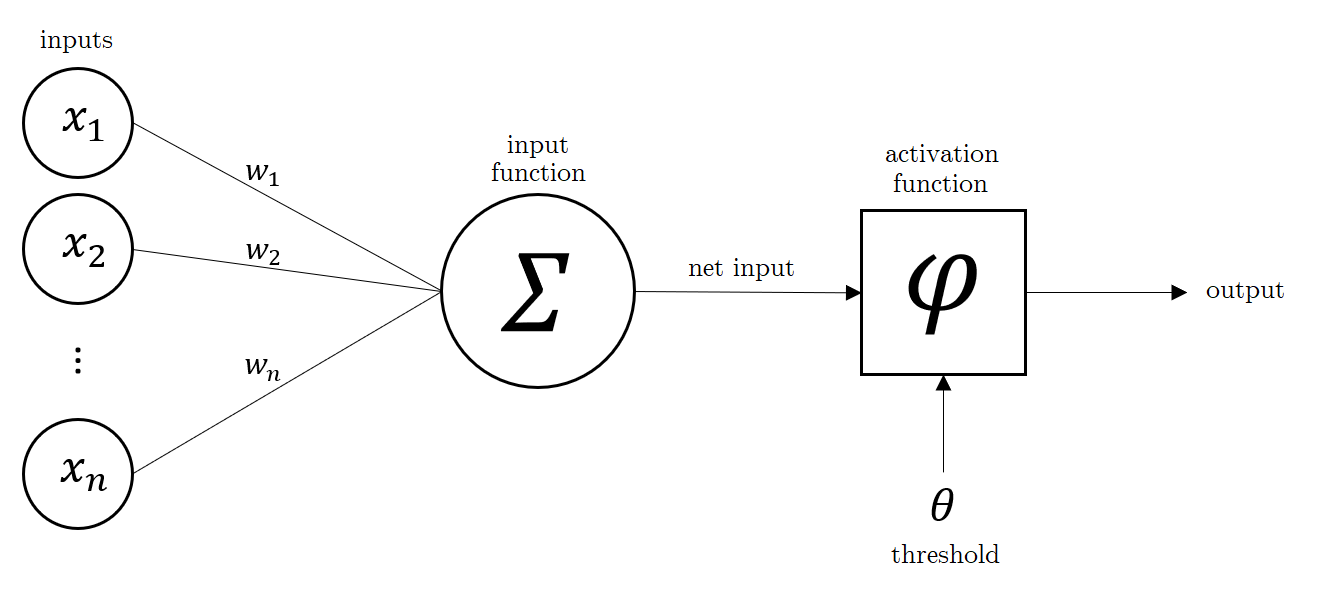
\includegraphics[width=0.7\textwidth]{images/perceptron}
    \caption{Perceptron}
    \label{fig:perceptron}
\end{figure}



\WIP{
\cite[p.~214f]{dlma14}
supervised learning provides discriminative power for pattern classification. need labelled data (ground truth) to train, meaning you need to provide examples for input with respective output. good for learning classification tasks.
unsupervised learning does not need labels. it intends to capture high-order correlation of the data. can be used to extract sparse representations or generate new data of same type.

\cite[pp.~125f]{nn_intro96}
training process is essentially updating the weights to achieve better matching prediction.

\cite[pp.~163ff]{nn_intro96}
training of NNs require error function to measure deviation from prediction to desired output. error is then to be minimized during training to create best-matching predictions. Achieved by backpropagation algorithm which searches for minimum of error function using gradient descent. first a forward pass through the NN is done to get all outputs and activations from all neurons. then you calculate for each individual neuron the effect it has for the total error. based on that you can adjust the weights between neurons to reduce the overall error.
}


\begin{itemize}
    \item compare training methods for deep learning (supervised, unsupervised, reinforcement learning)
    \item emphasize requirements and advantages of the different methods
    \item raise ideas how the methods can be used throughout the thesis
\end{itemize}

\subsection{Computer Vision Tasks}
There are many different tasks in computer vision for detecting and labelling objects in images. This section will give a brief summary of common tasks in the field. In addition, popular data sets with their scoring methods and suitable approaches to solving the problems are presented.

One of the easier tasks is called \emph{image classification}~\cite[p.~98]{DLbook16}. It is about choosing a matching category from a set of predetermined categories for a single image. To achieve that, recent approaches use convolutional neural networks as described in section~\ref{sec:cnn}. The output is a probability distribution which indicates the likelihood that the image will fit into a category. The category with the highest probability score can then be selected as the final label for the image. A popular data set for this task is the \emph{MNIST handwritten digits database}, that can be found in~\cite{mnist10}. To measure the performance of the solutions, the challenge recommends to compare the relative error rate of wrong labels in the test set.

The next level is to not only assign a label to an image, but also detect where the object in the image is located. Thus, this task is referred to as \emph{object localization}~\cite{rcnn14}. In addition to the category label, the output is extended by a rectangular bounding box that encloses the spatial extent of the object. This change allows to detect multiple objects in the same image, each with a category label and a (possibly overlapping) bounding box. There are different ways to solve this task, like for example bounding box regression~\cite{obj_detection13} or region proposal networks~\cite{ff-rcnn14}. The \emph{ImageNet} data set presented in~\cite{imgnet09} provides millions of images with prepared object categories and bounding boxes. The performance measurement for this data set is calculated by matching the proposed objects for an image and evaluating overlapping area in the bounding boxes.

Rectangular boxes are not very accurate for expressing the spatial extents of an object. Therefore, another task called \emph{semantic segmentation}~\cite{weakseg15} deals with pixel-level classification of an image. This determines a precise mask telling for each pixel of the image the object it belongs to. Since this is is one of the main tasks of this thesis, an in-depth discussion of modern solutions to this task follows in section~\ref{sec:ref_archs}. One data set to measure the performance of the various approaches is the Pascal Visual Object Classes as laid out in~\cite{pascal_voc15}. The scoring is done by calculating the \emph{intersection over union} (IoU), which gives the percentage of overlap for the predicted mask compared to the actual mask (see equation~\ref{eq:iou}).

\begin{equation}
    \label{eq:iou}
    \text{IoU} = \frac{\text{target} \cap \text{prediction}}{\text{target} \cup \text{prediction}}
\end{equation}

The last task to mention here for the sake of completeness is called \emph{instance segmentation}~\cite{mask-rcnn14}. Whereas previously only one category had to be assigned to each pixel, a distinction is now also made between pixels that belong to the same object category but different instances of an object. This task is quite challenging, as for example parts of an instance can be hidden by another instance of the same category, which leads to gaps in the mask. \emph{Mask R-CNN}~\cite{mask-rcnn14} is a widely used meta-algorithm for solving this task. It combines region proposals used for object localization with semantic segmentation processes. A great data set for this challenge is the \emph{Microsoft Common Objects in Context} set, which can be found in~\cite{coco15}.

\begin{figure}
    \newcommand{\imgWidth}{0.4\textwidth}
    \centering
    \hfill
    \begin{subfigure}{\imgWidth}
        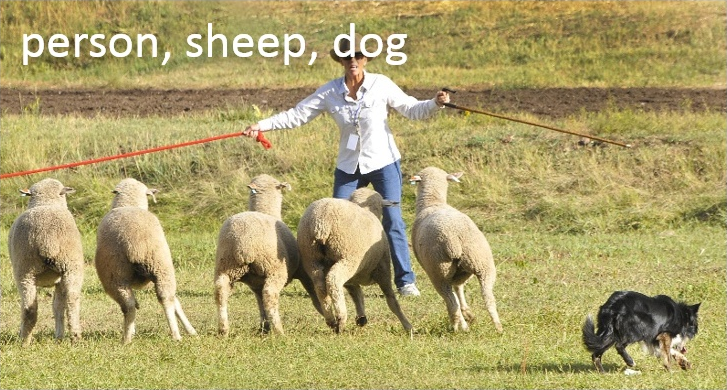
\includegraphics[width=\textwidth]{images/vision_task_1}
        \caption{Image Classification}
        \label{fig:cv_task_imgclass}
    \end{subfigure}
    \hfill
    \begin{subfigure}{\imgWidth}
        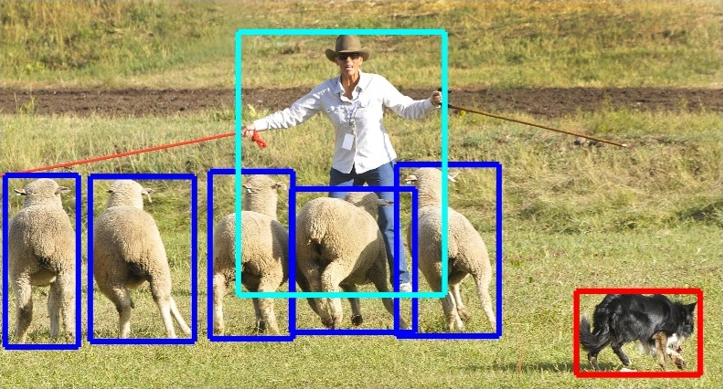
\includegraphics[width=\textwidth]{images/vision_task_2}
        \caption{Object Localization}
        \label{fig:cv_task_objloc}
    \end{subfigure}
    \hfill

    \hfill
    \begin{subfigure}{\imgWidth}
        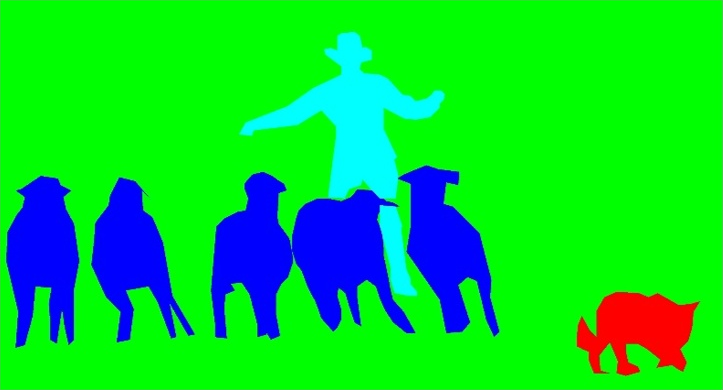
\includegraphics[width=\textwidth]{images/vision_task_3}
        \caption{Semantic Segmentation}
        \label{fig:cv_task_semseg}
    \end{subfigure}
    \hfill
    \begin{subfigure}{\imgWidth}
        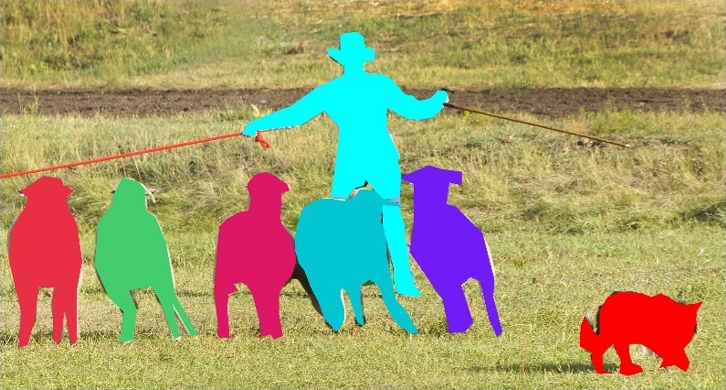
\includegraphics[width=\textwidth]{images/vision_task_4}
        \caption{Instance Segmentation}
        \label{fig:cv_task_inseg}
    \end{subfigure}
    \hfill

    \caption{Computer Vision Tasks~\cite{coco15}}
    \label{fig:cv_tasks}
\end{figure}

To give a brief summary, figure~\ref{fig:cv_tasks} depicts a visual representation of all the tasks mentioned above.

\subsection{Convolutional Neural Networks}
\label{sec:cnn}

One subclass of neural networks is called \emph{Convolutional Neural Network} (CNN) ~\cite[p.~359]{praxiseinstieg_ml17}. These types of networks show great results on data with a grid-like topology. Thus, they are often used for processing of image or video data. In traditional neural networks the layers are often densely connected, meaning every neuron of one layer is connected to every neuron in the next layer. For grid-like data this is not very efficient, because cells close to each other are often more likely to be correlated. Instead of dense connections, CNNs use operations called \emph{convolution} and \emph{pooling}, which allow to take spatial properties of the input data into account. The following sections explain the commonly used operations in CNNs.
% TODO: name general architecture with conv, pool and fc layers

\subsubsection{Convolution}
\label{sec:convolution}
% TODO: be more precise with input/output of neurons
\emph{Convolution} is a mathematical operation that uses weighted point-by-point multiplication of two matrices resulting in a scalar value. The concept is shown in figure~\ref{fig:convolution}. The notation $n_{k,~i,~j}$ represents a neuron at row~$i$ and column~$j$ in layer~$k$. For a convolutional layer, neuron $n_{k,~i,~j}$ is connected to all neurons $n_{k-1,~i,~j}$ to $n_{k-1,~i + f_w -1,~j + f_h -1}$. The neurons in layer~$k-1$ are therefore called receptive field of $n_{k,~i,~j}$ with a kernel width of $f_w$ and kernel height of $f_h$.~\cite[p.~361 f]{praxiseinstieg_ml17}

% TODO replace image with proper illustration
\begin{figure}[h]
    \centering
    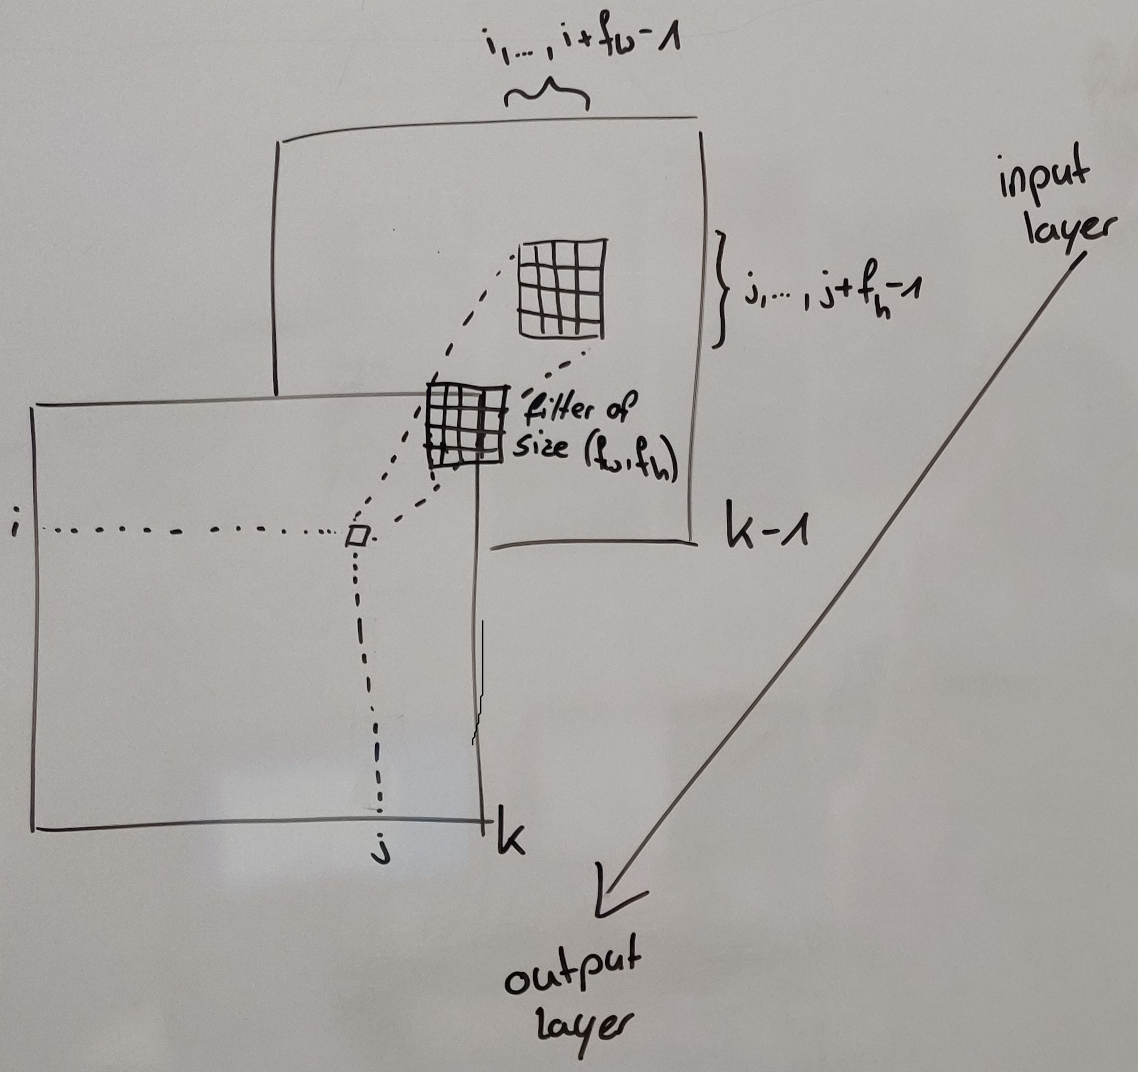
\includegraphics[width=0.6\textwidth]{images/convolution_template}
    \caption{Receptive field of a convolution operation}
    \label{fig:convolution}
\end{figure}

There are different ways to handle the edges of the grid. If no special action is taken, the output layer will be smaller in terms of edge length. For this reason \emph{zero padding} is often used to enlarge the input layer before convolution is performed. With an appropriate padding it is possible to preserve the width and height of the layer. Another parameter that affect the size of the output layer is called \emph{stride}, that controls the distance between to neighbouring receptive fields.~\cite[p.~361]{praxiseinstieg_ml17}

The trainable parameters in a convolution layer are the weights and biases used for the matrix multiplication introduced earlier. One specific set of weights and biases is called a \emph{filter}. It is responsible for detecting one single feature of the input layer. The output of a filter is thus referred to as \emph{feature map}. To inspect multiple features of the input, a convolution layer usually consists of multiple filters that are trained and calculated independently. In the end, the output of a convolution layer are multiple feature maps, each highlighting one single feature of the input.~\cite[p.~363 f]{praxiseinstieg_ml17}

As stated by Goodfellow et al.\ in~\cite{DLbook16} the convolution operation has some properties that are highly valuable to build an efficient and powerful neural network. Compared to traditional neural networks, convolution layers have only few connections between to subsequent layers. This is because the kernel is much smaller than the input. Especially for images, which can have millions of pixels, this helps to reduce the number of parameters to train.  Furthermore, the convolution reuses the same parameters for an entire feature map. Besides increasing the statistical efficiency of the model, it also makes the operation equivariant to translation in the input.

% TODO: explain the above section in more detail?
\begin{comment}
    \cite{DLbook16}
    330: NN use only matrix multiplication. meaning every output unit of one layer interacts with the all input units of the next layer. convolution leverages sparse interactions. for example images can have millions of pixels, but to detect edges it is enough to only look at a few pixels at a time. thus we can have a kernel smaller than the image size resulting in fewer parameters. This reduces memory requirements of the model and increases statistical efficiency.

    331, 333: another advantage is parameter sharing. with matrix multiplication you usually have a weight matrix, where each value is used only once. convolution operation uses parameter sharing, because one kernel is applied multiple times on the same image. and since kernel is smaller than image, it again reduces number of parameters by a significant amount.

    334f: due to parameter sharing, convolution operation is equivariant to translation. Meaning, if you move parts of the input convolution will still give you the same output, just with the moved detection. This is especially helpful for working with images, as object might be in different locations of the image, but should still be realized.
\end{comment}

\subsubsection{Pooling}
\label{sec:pooling}
Unlike convolution, which is used to extract features from the input, \emph{pooling} removes information from the data to reduce the number of parameters and also to prevent overfitting. The procedure of pooling is similar to convolution. However, it does not use matrix multiplication but instead performs a predefined mathematical function on the input matrix. While any function can be used for the pooling operation, most of the times it is the $\max$ function. Thus, it reduces the available information but still keeps the most important activations.~\cite[p.~369 f]{praxiseinstieg_ml17}

Because the function to use is predefined, pooling layers do not contain any trainable parameters. But still they are configurable with the same hyperparameters as convolution layers, namely kernel size, stride and padding. In addition, you can not only do pooling along the two axis of the input, but also along the third axis, which are the feature maps.~\cite[p.~370]{praxiseinstieg_ml17}

% TODO replace image with proper illustration
\begin{figure}[h]
    \centering
    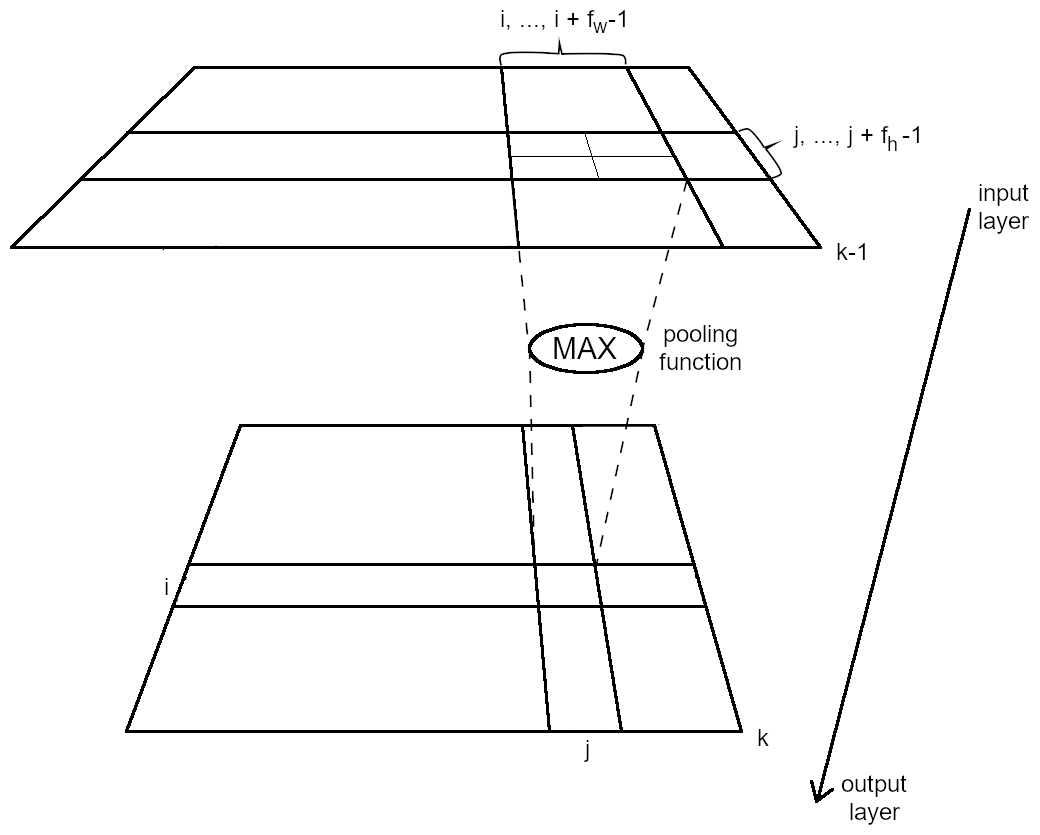
\includegraphics[width=0.6\textwidth]{images/maxpool_template}
    \caption{Max pooling}
    \label{fig:pooling}
\end{figure}

\WIP{\cite{spp15}
special kind of pooling used in CNNs called spatial pyramid pooling (SPP). Used to overcome a common issue in image processing which is size and aspect ratio. Convolution and pooling layer are not impaired by varying image sizes, but FC layers at the end are. Thus, images have to be scaled/warped to fit given input size.

SPP usually applied instead of last pooling layer before FC layers. maintains spatial information by having spatial bins in proportion to image size. multiple levels are used (thus pyramid). level 0 is doing global max pooling, resulting in 1 value for every feature map. level 1 has 4 bins (2x2 structure) and level 2 has 16 bins (4x4 structure). all they do is max pooling inside every bin. this leads to fixed-length outputs for arbitrary input sizes. Figure~\ref{fig:spp_pooling} shows SPP layer in action.
}

\begin{figure}[h]
    \centering
    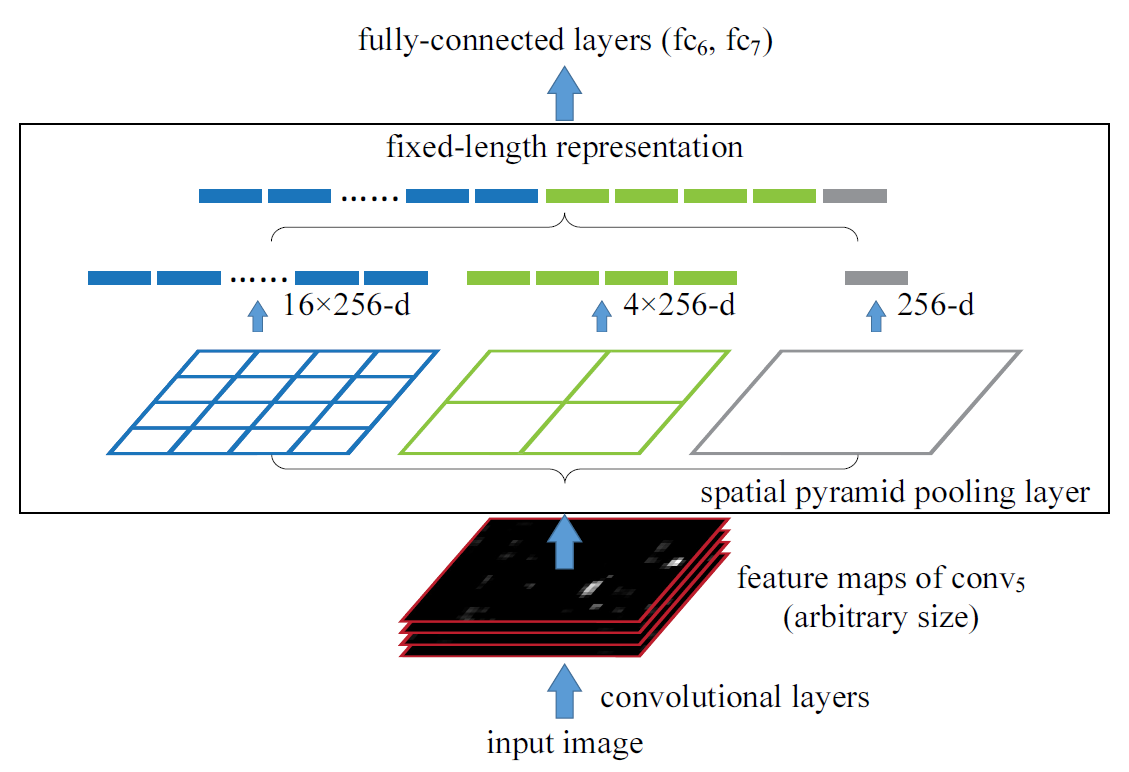
\includegraphics[width=0.6\textwidth]{images/spp_pooling}
    \caption{Spatial pyramid pooling}
    \label{fig:spp_pooling}
\end{figure}

\subsubsection{Other Important Concepts}
\begin{itemize}
    \item Batch Normalization
    \item ReLU Activation
\end{itemize}

\WIP{
reducing labelling effort with \cite{scribble16}. only provide scribbles instead of pixel-level segmentation masks.

\cite{decoupled15}
semi-supervised learning approach. combine small number of strong annotations with large number of weak annotations. few images with full segmentation masks are enough, but need many images with labelled classes. authors separate classification from segmentation network. can make use of existing classification networks. add a bridge layer to extract activation map from classification network. this is fed into segmentation network, which uses upsampling to output pixel-level segmentation mask.
}

\subsection{Reference Architectures}
\label{sec:ref_archs}
\begin{itemize}
    \item make clear why it is convenient to use reference architectures
\end{itemize}

\WIP{\cite{fcn15}
CNN play key role in computer vision tasks. NN in general computes nonlinear function, fcn computes nonlinear filter. therefor, can handle any input size and produce corresponding output size (keep spatial dimensions). Authors take existing classification architectures and transform them to fcn approach. last fully-connected layers are replaces by convolutional layers. output is then a coarse classification heatmap (smaller than input image).

to go back to full resolution, authors describe upsampling (deconvolution). This is convolution as described in \ref{sec:convolution}, but with fractional stride. this leads from coarse to dense prediction for pixels. Following architectures utilize the idea of FCN and upsampling to make dense predictions for segmentation maps.
}

\subsubsection{U-Net Architecture}
%TODO: go more into detail on the training and the results they achieved
In 2015, Ronneberger et al.\ introduced an architecture called \emph{U-Net} which they recommended for binary segmentation of biomedical images~\cite{unet15}. As can be seen in figure~\ref{fig:unet_architecture}, this name derives from the U-shape of the network model. It consists of a contracting path in the beginning, in which convolution and pooling layers are used to condense the input. The second half forms an expansive part, that uses convolution and upsampling layers to go back to the scale of the original image. Note that the outputs of the convolution layers in the contracting path are cropped and then concatenated to the input layers with the corresponding size in the expansive path. By doing that, the expansive layers still retain enough information from the original input to deliver a precise segmentation.

\begin{figure}[h]
    \centering
    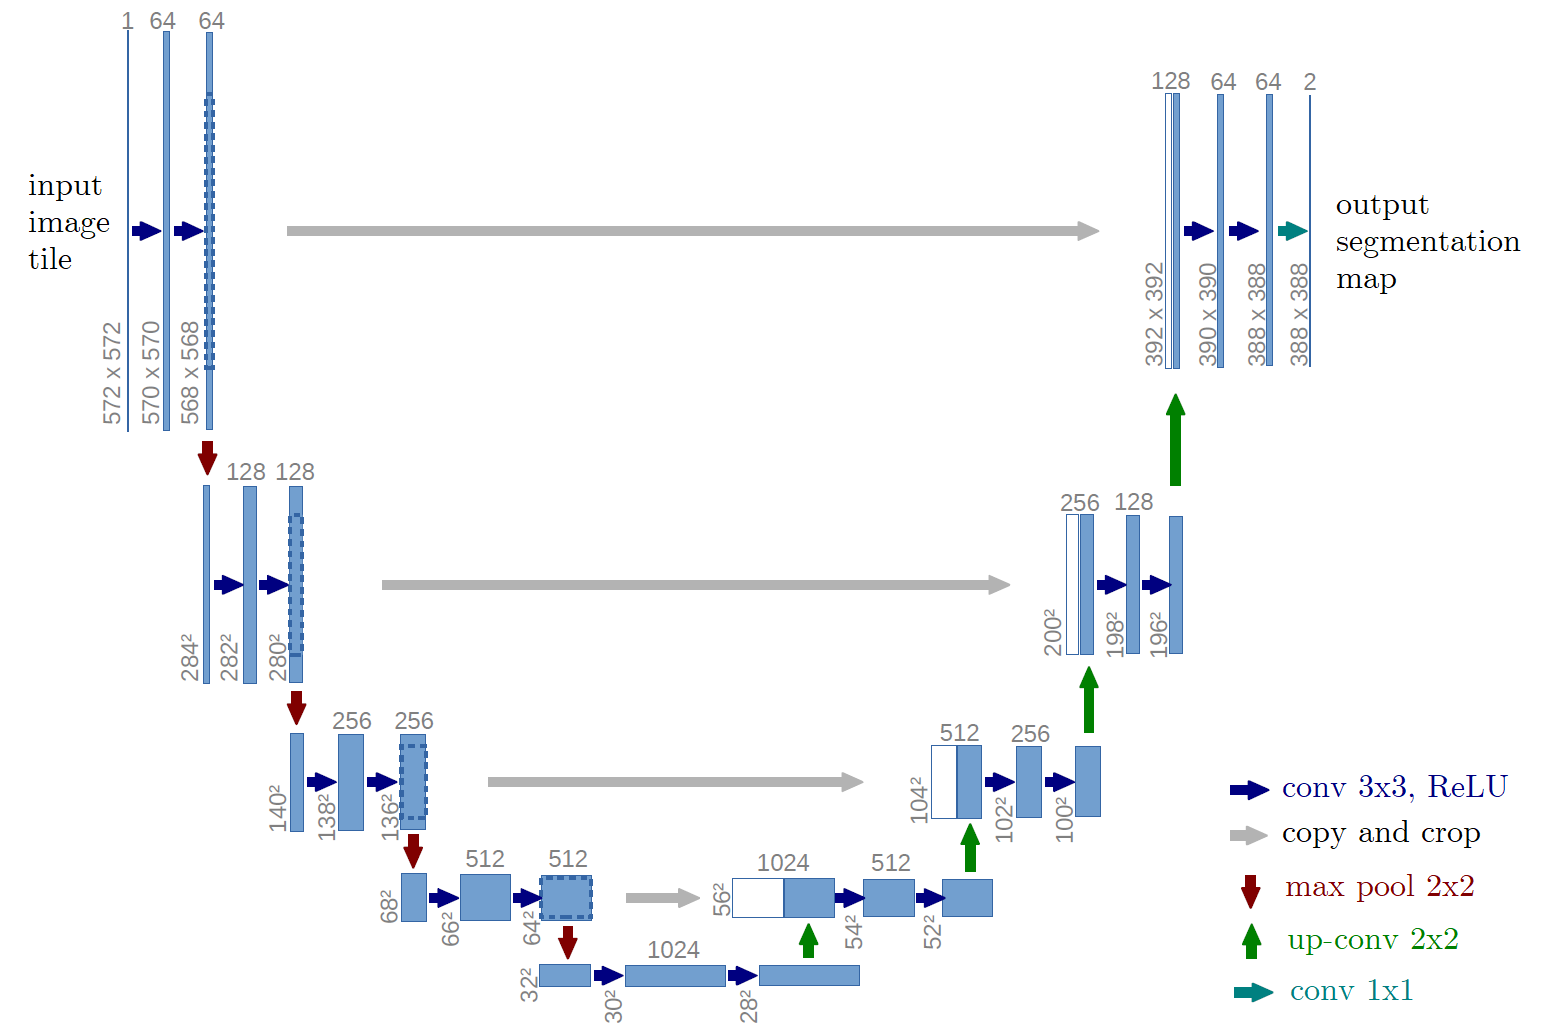
\includegraphics[width=0.9\textwidth]{images/u-net-architecture}
    \caption{U-Net Architecture \cite{unet15}}
    \label{fig:unet_architecture}
\end{figure}

The U-Net architecture contains neither fully connected layers nor do they use padding for the edges. Thus, the segmentation map has a lower resolution that the original image, because it only contains pixels for which the full context is available. By using a tiling strategy with overlapping tiles, this approach can produce seamless segmentation maps for input images of arbitrary size. For the edges of the input image, Ronneberger et al.\ suggest a mirroring strategy to extrapolate the missing context.~\cite{unet15}


\subsubsection{DenseNet Architecture}
As the depth of CNN architectures tends to increase, a new challenge arose regarding the training of those networks. Since the hidden layer can be very far away from the input and output layers, the values and gradients passed between the layers can get lost on the way. In an attempt to solve this, Huang et al.\ came up with the idea to directly connect all layers with matching feature map sizes. They published their architecture under the name \emph{DenseNet} in~\cite{densenet18}.

Huang et al.\ see the values passed between layers as a state. To access the state of one of the early layers in the network with a subsequent layer, all the layers in between have to pass the state unchanged, thus creating redundancy. With the DenseNet architecture, the state of all previous layers is explicitly passed to subsequent layers. This means, the network now differentiates between information that originates from an earlier layer and new information found in the current layer. It allows to keep the convolution layers narrow, because each layer only adds information, but never changes information that was previously acquired. This concept leads to having fewer trainable parameters and an improved flow of gradients, which both reduce the effort for training the network.~\cite{densenet18}

\begin{figure}[h]
    \centering
    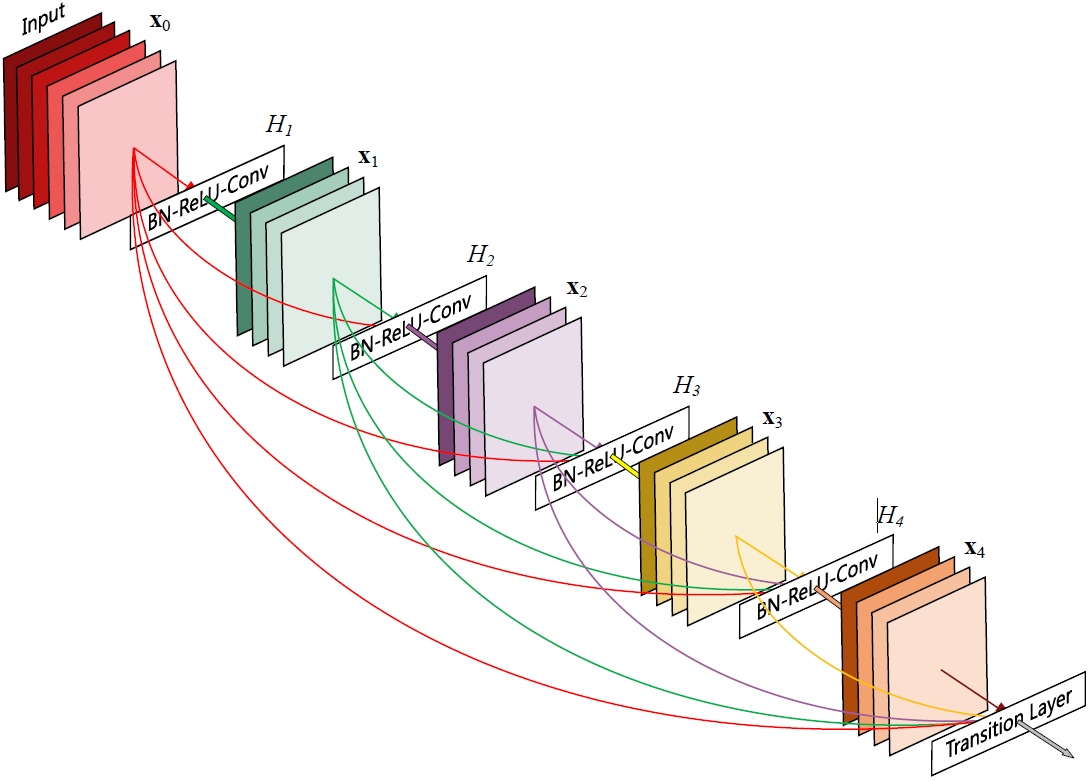
\includegraphics[width=0.7\textwidth]{images/dense-net-architecture}
    \caption{Densely Connected Convolutional Architecture~\cite{densenet18}}
    \label{fig:densenet_architecture}
\end{figure}

To add the connections between the layers, the authors simply concatenate the feature maps. Thus, it is not possible to connect layers which feature maps are of different size. To still be able to use pooling layers to condense the information in the network, the authors introduce a component called \emph{dense block} as illustrated in figure~\ref{fig:densenet_architecture}. Inside of a dense block, they apply dense connections between the convolution layers. In between two consecutive dense blocks, there is a \emph{transition layer}, which is formed by a convolution and an average pooling layer. Ultimately, the overall architecture of a DenseNet consists of several independent dense blocks separated by transition layers, eventually concluded by a fully-connected layer.

\subsubsection{Mask R-CNN}
\label{sec:mask-rcnn}

\WIP{
\cite{rcnn14}
image classification not sufficient for segmentation, because of missing localization. CNN combined with region proposals leads to R-CNN. Is not a fixed architecture, but more a meta algorithm whose implementation can vary. Architecture consists of three modules: category independent region proposals with selective search (fast mode). This outputs regions of interest (RoI). Affine image warping to make all regions same size, then passed through CNN architecture. This extracts fixed-length feature vector for each region. Then, support vector machines used to compute probabilities for every class. Overall Output is class prediction and offset for proposed region. visualized in figure~\ref{fig:rcnn_architecture}

This architecture had performance issues, training/test took very long. first improved in \cite{f-rcnn14} by first computing feature maps. Then identify RoIs directly in feature map and use RoI pooling (special kind of SPP pooling, only one pyramid layer) to generate fixed-size output layer. Then again, FC layers for classification and bounding box regression. This way, a lot of time is saved because convnet is only used once.

After that, selective search was the limiting factor in speed, so \cite{ff-rcnn14} examined a new way to get region proposals. This leads to region proposal networks (RPN), which shares convolutional layers with CNN. Thus the cost to compute region proposals is very small during test time. Allows for object detecting near real-time.
}

\begin{figure}[h]
    \centering
    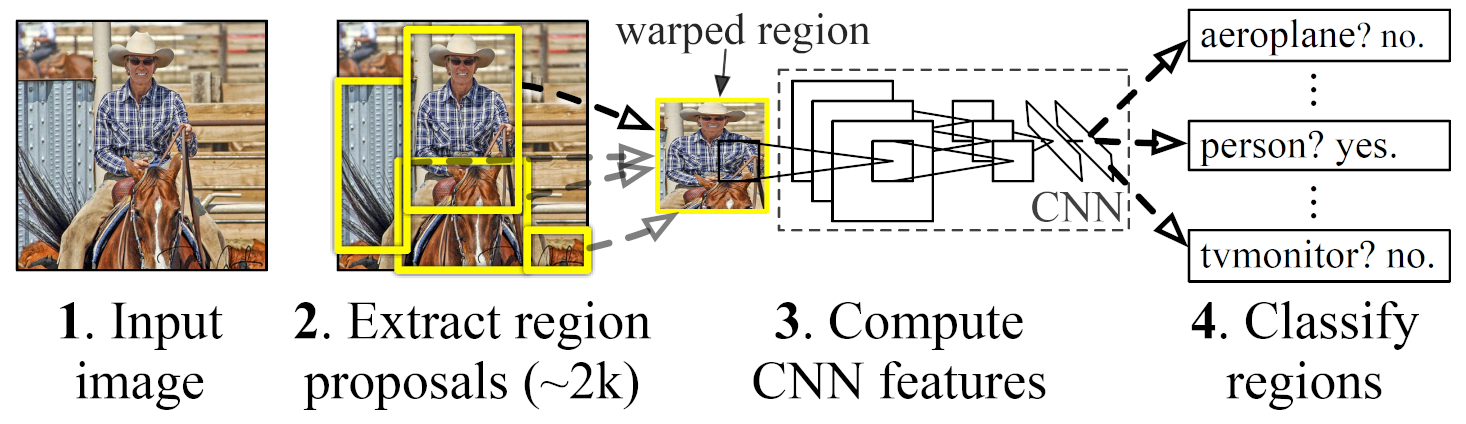
\includegraphics[width=0.7\textwidth]{images/rcnn}
    \caption{R-CNN architecture~\cite{rcnn14}}
    \label{fig:rcnn_architecture}
\end{figure}

\WIP{
Still, Faster R-CNN has only Object localization. Another extension called Mask R-CNN~\cite{mask-rcnn14} introduced instance segmentation for R-CNN. Uses identical first stage with RPN. Then adds another path for mask prediction besides the class and bounding box predictions. In contrast to other architectures, class prediction and mask predication are independent. Binary Masks are predicted for every class without competition.

RoI pooling is not sufficient for masking, because of quantization described in \cite{f-rcnn14}. it is okay for classification, but introduces misalignment on pixel level which makes it unusable for segmentation. Thus, \cite{mask-rcnn14} came up with RoI Align layer, that has no quantization by avoiding rounding and using bilinear interpolation.
}

\subsection{Architecture Comparison}
Interesting for architecture comparison: \cite{imseg_architecures}

\begin{itemize}
    \item point out the common characteristics and differences of the architectures
    \item compare use cases of the architectures and how they perform on them
\end{itemize}

\newpage